\subsection{Using the Landau approach} 
We can study the behavior of $f(m)$ more closely by Taylor expanding. From here on out, we'll think of $m$ in a more general sense, as something that we'll call an 'order parameter', and see how $f$ changes. 

Using the expansions 
\[ 
	\log (1+ m) = m - \frac{ m^2}{2} + \frac{m^3}{ 3} - \frac{ m^4}{ 4}  + \dots 
\] 
One can easily verify that up to $O(m^ 4) $, we have 
\[ 
	(1 + m ) \log ( 1 + m) + ( 1 - m ) \log ( 1 - m ) \simeq  m ^2 + \frac{ m^4}{ 6} 
\] 
Thus, we have an expansion for our expression 
\[
	f(m ) =  - T\log 2  - Bm + \frac{1}{ 2} ( T  - Jq ) m^ 2 + \frac{T}{ 12} m^4 
\] 

\subsubsection*{The case when $ B = 0 $}
We'll now take a look at the equilibrium states of, where $ \partial f / \partial m  =0 $. In the case of $B = 0 $, we have a quartic that looks qualitatively different depending on whether $ T > Jq $ or whether $T < Jq $. This is shown in the graphs 
\begin{figure}
	\centering 
	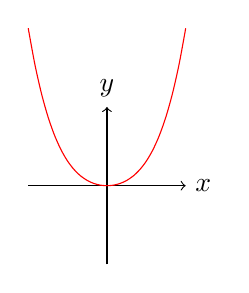
\begin{tikzpicture} 
		\draw[->] ( - 1, 0 ) -- (1, 0 ) node[right] {$x$}; 
		\draw[->] (0, -1) -- ( 0, 1) node[above] {$y$}; 
		\draw[scale=1, domain=-1:1, smooth, variable=\x, red] 
			plot ({ \x}, {\x * \x * \x * \x + \x * \x  } );  
	\end{tikzpicture} 
	\quad 
	\begin{tikzpicture} 
		\draw[->] ( - 1, 0 ) -- ( 1, 0 ) node[right] {$x$}; 
		\draw[->] (0, -1) -- ( 0, 1) node[above] {$y$}; 
		\draw[scale=1, domain=-1:1, smooth, variable=\x, red] 
			plot ({ \x}, {\x * \x * \x * \x  - \x * \x  } );  
	\end{tikzpicture}

	\caption{ Here we've shown plots where $T > T_c$ on the left versus when $T< T_c$} 
\end{figure} 
In the case where $T > T_c $, our minimum point is at $m = 0$ as shown in the graph, which means that we have no average magnetisation. For this reason, we call this a disordered state. 
When $T < T_c$, we have that the system that settles at either minimum point. We can calculate this minimum point explicitly by differentiating by solving for $f'(m ) $ to get that our minimum points are 
\[ 
m_0 = \pm \sqrt{ \frac{ 3 ( T_c - T ) }{ T } } 
\] 
This is our first example of a phase transition; when a physical quantity (in this case, average magnetisation), depends discontinuously on some parameter. We define an nth order phase transition when the nth derivative of the equilibrium value is discontinous when we differentiate it by some parameter.In other words, when the function $f'(\mu) = f( \mu, m_0 )$ is discontinuous when we differentiate it n times with respect to $\mu$, then do we have a phase transition. In this example, if we substitute our values of $m_0$ back into $f$, then 
\[ 
f(m_0, T) = \begin{cases} 
		0 & T > T_c \\ 
		 - \frac{3}{ 4} \frac{ ( T - T_c)^2 }{ T }  & T< T_c 			\end{cases} 
\] 
At $ T = T_c$, we have that $f( m_0, T )$ and $\frac{ df }{ dT } $ are continuous, but we have a discontinuity at $\frac{ d^2 f}{ dT^2 } $. 
Thus, our phase transition is a second order phase transition. 
We can also see this discontinuity exhibited when we examine heat capacity. 

Our heat capacity is defined as our change in average energy as temperature changes
\[ 
\frac{ d \langle E \rangle }{ dT}  = c
\] 
But we can calulate average energy in terms of our partition function $Z$, which is given by 
\[ 
\langle E \rangle = \frac{ - \partial \log Z }{ \partial B} 
\] 
We use the chain rule to express derivatives in $T$ as derivatives in $\beta$
\[ 
\frac{d}{ dT} = \frac{ d \beta} { dT } \frac{ \partial }{ \partial \beta} =  - \beta^ 2 \frac{ \partial }{ \partial \beta} 
\] 
Hence our heat capacity is given by the formula 
\[ 
c = \beta^2 \frac{ \partial^2 \langle \log Z \rangle}{ \partial \beta^2 } \] 
Now, with our saddle point approximation, we know that 
\[ 
\log Z = - \beta N f(m_{min} ) \implies \log Z =  - \beta N f(m_{min}) = \begin{cases} 
0 & T > T_c \\
\beta N \frac{ 3}{ 4} \frac{ ( T - T_c)^2 }{ T^2 }  & T < T_c 
\end{cases} 
\]  
In the case when $ T < T_c $, we have that setting $T = 1 / \beta $ gives us that 
\[ 
\log Z = \frac{ 3}{ 4} N ( 1 - 2 T_c \beta + T_c^2 \beta^2 ) \implies c = \frac{3}{ 2} N T_c^2 \beta^2 
\] 
Hence, as $T \rightarrow T_c$, we have a discontinuity in our heat capacity \[ 
C = \begin{cases} 
0 & T \rightarrow T_c^- \\
\frac{3}{2} N & T \rightarrow T_c^+ 
\end{cases} 
\] 
Since this involves a discontinuity in a second derivative of $f(m_{min})$ ( in this case $\beta$ ), this is a second order phase transition. 


\subsubsection*{The case when $B \neq 0 $} 
Now, in the case where $B \neq 0$ and we have our free energy given by 
\[ 
f(m) =  - Bm + \frac{1}{ 2}( T - T_c )m^2 + \frac{T}{ 12} m^4 + \dots \] 
In the case where $T < T_c$, we already have two minimum points, but as the graphs show we have a global minimum at a specific point depending on the sign of $B$. This is shown in the graphs below, where when $B>0$ our equilibrium magnetisation lies at $m_0 > 0$, and when $ B < 0 $ our equilibrium magnetisation lies at at $m_0 < 0$. 

\begin{figure}[h]
\centering
\begin{tikzpicture}[scale=0.7]
\begin{axis}[ 
xlabel=$m$,
ylabel={$f(m)$}, 
axis x line=center,
axis y line=center,
ticks=none, 
no markers, 
clip=false 
] 
\addplot { -  5 * x - 2 *  x^2 + 0.5 *  x^4}; 
\end{axis}
\end{tikzpicture} 
\quad
\begin{tikzpicture}[scale=0.7]
\begin{axis}[ 
xlabel=$m$,
ylabel={$f(m)$}, 
axis x line=center,
axis y line=center,
ticks=none, 
no markers, 
clip=false  
] 
\addplot { +  5 * x - 2 *  x^2 + 0.5 *  x^4}; 
\end{axis}
\end{tikzpicture}

\caption{Our global minimum depends on the sign of $B$ this time} 

\end{figure} 

